%%%%%%%%%%%%%%%%%%%%%%%%%%%%%%%%%%%%%%%%%%%%%%%%%%%%%%%%
%%%%%%%%%------RMIT SPACE POSTER------------%%%%%%%%%%%%
%%%%%%%%%%%%%%%%%%%%%%%%%%%%%%%%%%%%%%%%%%%%%%%%%%%%%%%%
%%%%%%%%%%%%%%%%%%%%%%%%%%%%%%%%%%%%%%%%%%%%%%%%%%%%%%%%
% a0poster Portrait Poster
%
% The a0poster class was created by:
% Gerlinde Kettl and Matthias Weiser (tex@kettl.de)
% 
% License:
% CC BY-NC-SA 3.0 (http://creativecommons.org/licenses/by-nc-sa/3.0/)
%
% Author/Designer: Timothy Kodikara
%
%% Note: CRC and SERC logos are included in the /figures folder if you might want to use them.
%%%%%%%%%%%%%%%%%%%%%%%%%%%%%%%%%%%%%%%%%
%----------------------------------------------------------------------------------------
%	PACKAGES AND OTHER DOCUMENT CONFIGURATIONS
%----------------------------------------------------------------------------------------
\documentclass[a0,portrait]{a0poster}
%%
\usepackage[top=5cm, bottom=0.3cm, left=5cm, right=3cm]{geometry}
\usepackage[compact]{titlesec}
\usepackage{multicol} % This is so we can have multiple columns of text side-by-side
\columnsep=100pt % This is the amount of white space between the columns in the poster
\columnseprule=15pt % This is the thickness of the blue line between the columns in the poster
\usepackage[svgnames]{xcolor} % Specify colors by their 'svgnames', for a full list of all colors available see here: http://www.latextemplates.com/svgnames-colors
%\usepackage{times} % Use the times font
\usepackage{palatino} % Uncomment to use the Palatino font
\usepackage{xkeyval}
\usepackage{graphicx} % Required for including images
\setlength{\abovecaptionskip}{5pt plus 5pt minus 3pt}
\graphicspath{{figures/}} % Location of the graphics files
\usepackage{booktabs} % Top and bottom rules for table
\usepackage[font=small,labelfont=bf]{caption} % Required for specifying captions to tables and figures
\usepackage{amsfonts, amsmath, amsthm, amssymb} % For math fonts, symbols and environments
\usepackage{csquotes}
\usepackage{wrapfig} % Allows wrapping text around tables and figures
%\usepackage[pdftex]{color}
\usepackage{multirow}
\usepackage{makecell}
\def\columnseprulecolor{\color{NavyBlue}}%
\usepackage{framed}
\colorlet{frameborder}{NavyBlue}
%----------------------------------------------------------------------------------------
%	POSTER HEADER 
%----------------------------------------------------------------------------------------
% The header is divided into three boxes:
% The widths of these boxes can be easily edited to accommodate your content as you see fit
\begin{document}
%\hspace*{0.2cm}
\begin{minipage}[c]{\linewidth}
\vspace{0.1cm}
\noindent\makebox[\textwidth][c]{
\begin{minipage}[c]{0.14\linewidth}
\vspace{0pt}\raggedright
\hspace{1cm}

\includegraphics[scale=1.3,width=\linewidth]{figures/logo.png}
\end{minipage}
\hfill
\begin{minipage}[c]{0.75\textwidth}
\centering
\Huge \color{Green} \textbf{IE643 Course Project}\\[0.5cm]
\Huge \color{NavyBlue} \textbf{Project Topic Name}\\[0.5cm]
\Large \color{NavyBlue} \textbf{Team Name}\\[0.5cm]
\large \color{Black} \textbf{Team Member Name 1 $^{1}$ (Roll Number), Team Member Name 2 $^{2}$} (Roll Number)\\[0.2cm] % Author(s)
\small \text{XXXX@iitb.ac.in$^{1}$, XXXXX@iitb.ac.in$^{2}$}\\
\large \color{Green} \textbf{}\\
\end{minipage}
%\hfill
\begin{minipage}[c]{0.145\textwidth}
\vspace{0pt}\raggedleft

\includegraphics[scale=1.3,width=\linewidth]{figures/IE643-Logo.pdf}
\hspace{1cm}
\end{minipage}}
\\[0.1cm]%
% A bit of extra whitespace between the header and poster content
%----------------------------------------------------------------------------------------
\color{NavyBlue}\setlength\FrameRule{25pt}
\begin{framed}
\vspace{0.5cm}
\begin{multicols}{2} % This is how many columns your poster will be broken into, a portrait poster is generally split into 2 columns
%----------------------------------------------------------------------------------------
%	Abstract
%----------------------------------------------------------------------------------------
\color{Black}
\section*{Abstract}
Short paragraph (Max 4-5 lines)

%----------------------------------------------------------------------------------------
%	INTRODUCTION
%----------------------------------------------------------------------------------------


\section*{Introduction}
\begin{itemize}
	\item Crisp Bullet Points.
\end{itemize}
\vspace{-\baselineskip}
\begin{center}
\hspace*{\fill}
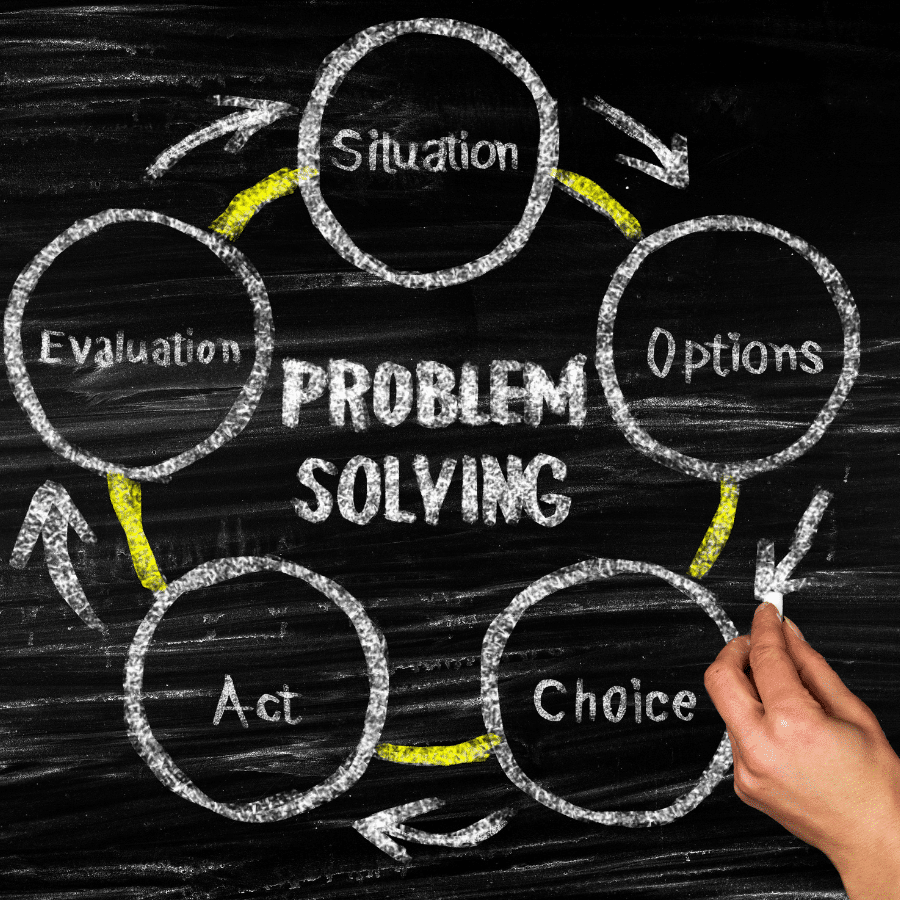
\includegraphics[width=0.5\linewidth]{figures/Intro.png}
\captionof{figure}{\color{Blue}Sample Caption}
\label{Intro}
\end{center}
We outline our major \textbf{contributions} below:
\vspace{-\baselineskip}\\
\begin{itemize}
	\item Crisp Bullet Points.
\end{itemize}

%----------------------------------------------------------------------------------------
%	Workflow
%---------------------------------------------------------------------------------------- 
\color{Black}
\section*{Workflow}
Figure \ref{workflow} illustrates the workflow,...
\begin{center}
	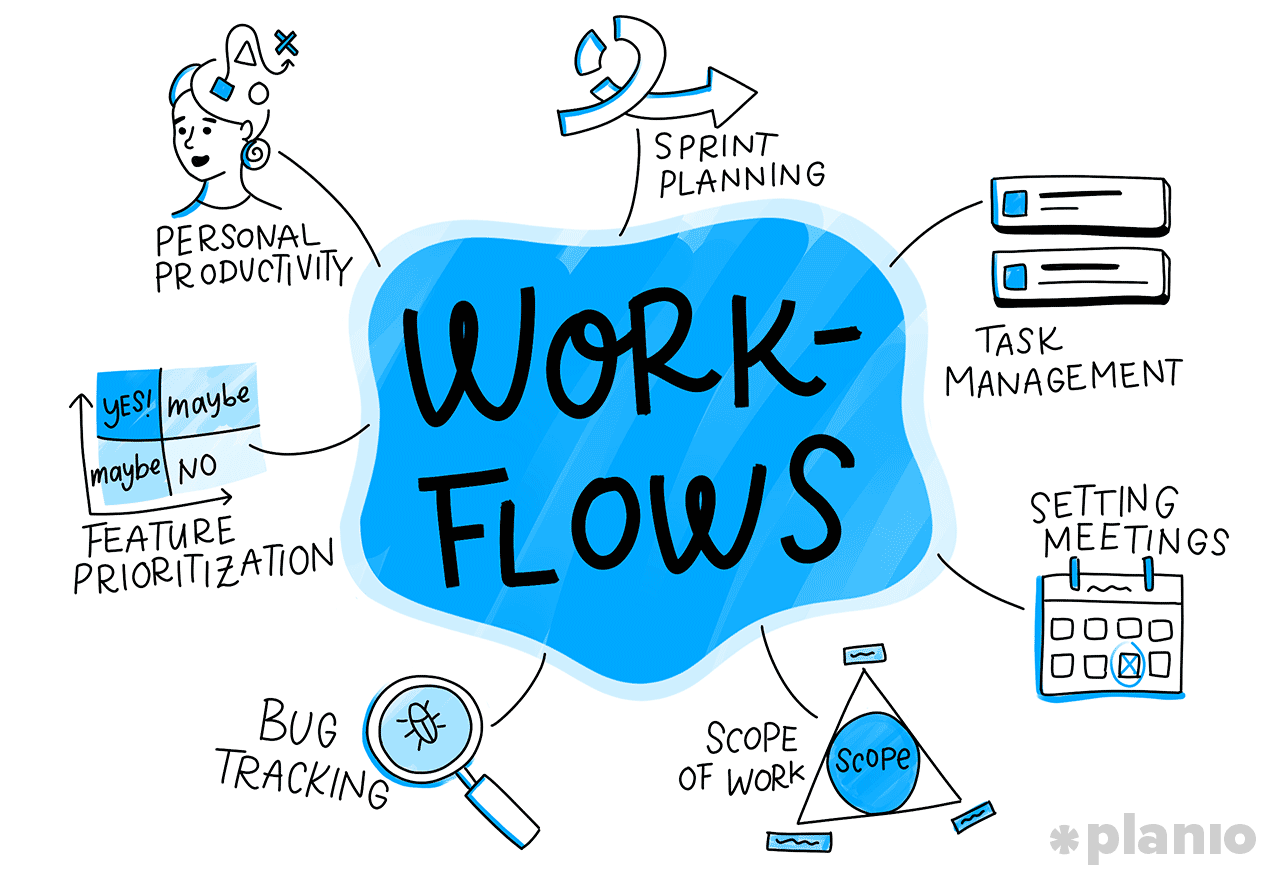
\includegraphics[width=0.95\linewidth]{figures/Workflow.png}
	\captionof{figure}{\color{Blue} Overall Workflow}
	\label{workflow}
\end{center}

%----------------------------------------------------------------------------------------
%	Methodology
%----------------------------------------------------------------------------------------

\section*{Methodology}
Figure \ref{Arch} illustrates the architecture,...
\begin{center}
	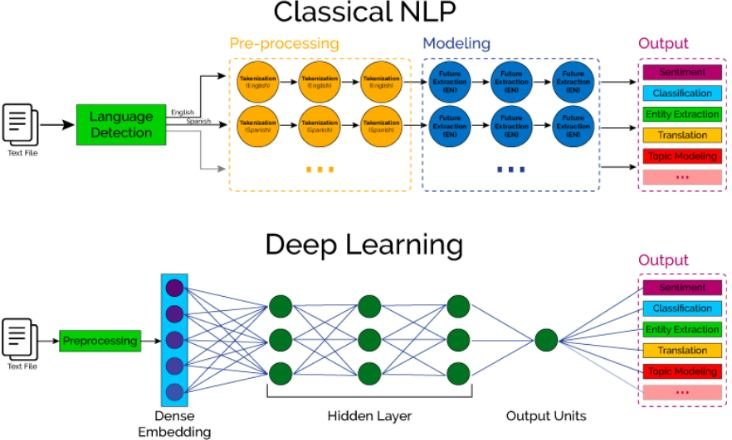
\includegraphics[width=0.95\linewidth]{figures/Deep-Neural-Network-Model.jpg}
	\captionof{figure}{\color{Blue} Overall Architecture}
	\label{Arch}
\end{center}

%----------------------------------------------------------------------------------------
%	Dataset Details and Experimental Setup
%----------------------------------------------------------------------------------------

\color{Black}
\section*{Dataset Details}
A tabulation of the dataset characteristics. Include most relevant data set details which are important for the project.

%----------------------------------------------------------------------------------------
%	Novelty Assessment
%----------------------------------------------------------------------------------------
\color{Black}
\section*{Novelty Assessment}
Illustrating the tasks attempted for novelty assessment and results obtained from the new experiments. 


%----------------------------------------------------------------------------------------
%	Results
%----------------------------------------------------------------------------------------

\color{Black}
\section*{Results}
Add both qualitative and quantitative results using suitable plots and tables describing the results obtained during the project. 

\begin{center}
	\scalebox{1.1}{
		\begin{tabular}{|c|c|c|c|c|c|c|}
			\hline
			Methods & metric-1 & metric-2 & metric-3 & metric-4 & metric-5 & metric-6\\
			\hline
			Model & 0.0 & ... & ... & ... & ... &  \\
			\textbf{Ours} & \textbf{0.0} & \textbf{0.0} & \textbf{0.0} & \textbf{0.0} & \textbf{0.0} & \textbf{0} \\
			\hline
		\end{tabular}
	\label{table}}\\
\captionof{table}{\color{Blue} Quantitative results}
	\vspace{-0.25in}
\end{center}
\vspace{0.25in}
Table \ref{table} showcase quantitative outcomes ...

%----------------------------------------------------------------------------------------
%	CONCLUSIONS
%----------------------------------------------------------------------------------------
\color{Black}
\section*{Conclusion}
\begin{itemize}
	\item Bullet points
	
\end{itemize}
%----------------------------------------------------------------------------------------
%	References
%----------------------------------------------------------------------------------------
\begin{thebibliography}{6}

\bibitem {U-net}
Ronneberger, O., et al.: U-net: Convolutional networks for biomedical image segmentation. In: Medical Image Computing and Computer-Assisted Intervention--MICCAI 2015: 18th International Conference, Springer (2015)

	
\end{thebibliography}
%----------------------------------------------------------------------------------------
%	ACKNOWLEDGEMENTS
%----------------------------------------------------------------------------------------
\section*{Acknowledgments}
\small \textnormal{We thank \textbf{}}

\section*{Github Link and Demo Video Link}
\vspace{-0.5cm}

\begin{center}
%	\framebox{
		\begin{minipage}{0.4\linewidth}
			\centering
			\textbf{Github Repository}\\[1ex]
			
\includegraphics[width=0.5\linewidth]{Sample_Code_QR.jpeg} % Replace with your QR code file
		\end{minipage}\hfill
		\begin{minipage}{0.4\linewidth}
			\centering
			\textbf{Demo Video Link}\\[1ex]
			
\includegraphics[width=0.5\linewidth]{Sample_Code_QR.jpeg} % Replace with your QR code file with your code demo interface link for users
		\end{minipage}
%	}
\end{center}


\end{multicols}
%\textcolor{NavyBlue}{\rule{\linewidth}{15pt}}
\vspace{0.5cm}
\end{framed}
\end{minipage}
%\hspace*{0.1cm}
\end{document}
%----------------------------------------------------------------------------------------
%%%%%%%%%%%%%%%%%%%%%%%%%%%%%%%%%%%%%%%%%%%%%%%%%%